% \input{"IAB/latex/TeX-Folienformat.tex"}
\input{"/Users/jonathanlatner/Google Drive/My Drive/IAB/latex/TeX-Folienformat.tex"}

\documentclass[t,8pt,utfx8]{beamer}
\usepackage{booktabs}
\usepackage{setspace}
\usepackage{parskip}
\usepackage{graphicx}
\usepackage{subcaption}
\setbeamertemplate{caption}[numbered]
\newcommand{\sprache}{\englisch}
\renewcommand{\thesubsection}{\alph{subsection})}
\usepackage[cal=pxtx, scr=dutchcal]{mathalpha}
\usepackage{forest}



\definecolor{codegreen}{rgb}{0,0.6,0}
\definecolor{codegray}{rgb}{0.5,0.5,0.5}
\definecolor{codepurple}{rgb}{0.58,0,0.82}
\definecolor{backcolour}{rgb}{0.95,0.95,0.92}


\usepackage{listings}

% Define style for R code
\lstset{
  language=R,
  basicstyle=\ttfamily\small,
  keywordstyle=\color{blue},
  stringstyle=\color{red},
  commentstyle=\color{green},
  showstringspaces=false,
  numbers=left,
  numberstyle=\tiny\color{gray},
  stepnumber=1,
  numbersep=5pt,
  breaklines=true,
  frame=single
}

\newcommand{\btVFill}{\vskip0pt plus 1filll}


\title{Buyer Beware: Understanding the trade-off between utility and risk in CART based models using simulation data}

\subtitle{Berlin, \newline 7-8. Oktober, 2024}

\author{Jonathan Latner, PhD \newline Dr. Marcel Neunhoeffer \newline Prof. Dr. Jörg Drechsler}

\newcounter{noauthorlines}
\setcounter{noauthorlines}{2} % Wert für 2 Autoren über 2 Zeilen. Ggf. anpassen

% %%%%%%%%%%%%%%
% Ende Anpassung
% %%%%%%%%%%%%%%

% \input{"IAB/latex/TeX-Folienformatierung_CD_2019"}
\input{"/Users/jonathanlatner/Google Drive/My Drive/IAB/latex/TeX-Folienformatierung_CD_2019"}

% Modify the section in toc template to enumerate
\setbeamertemplate{section in toc}{%
    \inserttocsectionnumber.~\inserttocsection\par
}

% use for subsections
% \setbeamertemplate{subsection in toc}{}
\setbeamertemplate{subsection in toc}{%
    \setlength{\parskip}{1mm}
        \hskip2mm -- \hskip1mm\inserttocsubsection\par
}


\usepackage{colortbl}
\definecolor{lightgray}{gray}{0.9}

\usepackage{listings} %include R code
\lstdefinestyle{mystyle}{
    backgroundcolor=\color{backcolour},   
    commentstyle=\color{codegreen},
    keywordstyle=\color{magenta},
    numberstyle=\tiny\color{codegray},
    stringstyle=\color{codepurple},
    basicstyle=\ttfamily\tiny,
    breakatwhitespace=false,         
    breaklines=true,                 
    captionpos=b,                    
    keepspaces=true,                 
    numbers=left,                    
    numbersep=5pt,                  
    showspaces=false,                
    showstringspaces=false,
    showtabs=false,                 
    columns=fullflexible,
    frame=single,
    tabsize=2
}
\lstset{style=mystyle}


\begin{document}


\frame[plain]{\titlepage}

\begin{spacing}{1.25}


%%%%%%%%%%%%%%%%%%%%%%%%%%%%%%%%%%%%%%%%
%%%%%%%%%%%%%%%%%%%%%%%%%%%%%%%%%%%%%%%%
\section{Introduction}\label{sec:introduction}
%%%%%%%%%%%%%%%%%%%%%%%%%%%%%%%%%%%%%%%%
%%%%%%%%%%%%%%%%%%%%%%%%%%%%%%%%%%%%%%%%

\begin{frame}[c,plain]
\vskip-4mm
\begin{beamercolorbox}[wd=\boxwidth,ht=22.11mm]{transparent}%
    \vfill%
    \usebeamerfont{title}%
    \leftinsert%
    \MakeUppercase{Section \ref{sec:introduction}: Introduction
} % <- Hier die Überschrift eintragen
\end{beamercolorbox}
\vskip-3mm
\pgfuseimage{rahmenlinie}
\end{frame}


\frame{\frametitle{Background}
\begin{itemize}
    \item We don't know.
    \item We think this idea is interesting.
    \item We think others should know about it.
    \item But we are still developing it.
    \item Thoughts and suggestions would be helpful.
\end{itemize}
}


\frame{\frametitle{Overview}
\begin{itemize}
    \item It is well established that there is a trade-off between utility and privacy when generating synthetic data
    \item Utility and privacy in CART based synthesizers is high (Little et al., 2022; Danker and Ibrahim, 2021)
    \item Therefore, CART models are less sensitive to this trade-off than other SDGs (i.e. higher utility, lower risk)
    \item Using simulation data (Reiter et al., 2014), we show that synthetic data from CART models are disclosive
    \item The problem:
    \begin{itemize}
        \item Disclosive in ways that are not observable with common privacy metrics
        \item It is possible to increase protection (by reducing utility)
    \end{itemize}
\end{itemize}
}

%%%%%%%%%%%%%%%%%%%%%%%%%%%%%%%%%%%%%%%%
%%%%%%%%%%%%%%%%%%%%%%%%%%%%%%%%%%%%%%%%
\section{Set up the attack}\label{sec:attack}
%%%%%%%%%%%%%%%%%%%%%%%%%%%%%%%%%%%%%%%%
%%%%%%%%%%%%%%%%%%%%%%%%%%%%%%%%%%%%%%%%
\begin{frame}[c,plain]
\vskip-4mm
\begin{beamercolorbox}[wd=\boxwidth,ht=22.11mm]{transparent}%
    \vfill%
    \usebeamerfont{title}%
    \leftinsert%
    \MakeUppercase{Section \ref{sec:attack}: Set up the attack
} % <- Hier die Überschrift eintragen
\end{beamercolorbox}
\vskip-3mm
\pgfuseimage{rahmenlinie}

Let me introduce a problem illustrating that CART is disclosive

\end{frame}

\frame{\frametitle{Setting up the attack}
\begin{itemize}
    \item Its a game between two entities.  
    \begin{itemize}
        \item The statistical agency has the data and wants to release it in a privacy preserving way.  
        \item The attacker wants to identify someone in the data (either membership or attribute inference).  
    \end{itemize}
    \item We assume the attacker has the following knowledge
    \begin{itemize}
        \item Knows the SDG model type (i.e. sequential CART).
        \item Knowledge of everyone in the data except one.  
        \item The 16 possible combinations that the last one could be.
    \end{itemize}
    \item The question: What can the attacker learn from a released synthetic data set about that individual they do not have knowledge of?
\end{itemize}
}

\frame{\frametitle{The original data: Simulate data with a unique record}

Borrowing from Reiter et al. (2014), we set the first 999 observations to be a random sample from a multinomial distribution for all combinations of $var1(0,1), var2(0,1), var3(0,1), var4(0,1)$ except ($var1=1,var2=1,var3=1,var4=1$), which we set to be the 1000$^{th}$ observation. 

\begin{minipage}{0.48\textwidth}
    \centering
    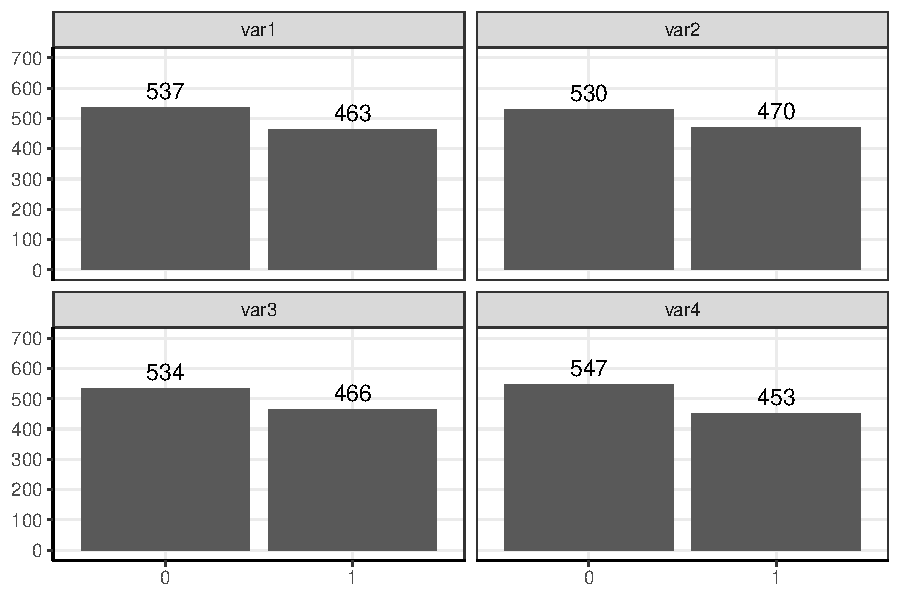
\includegraphics[width=\textwidth]{../../graphs/graph_numeric_frequency.pdf}
    \captionof{figure}{Frequency}
\end{minipage}
\hfill
\begin{minipage}{0.48\textwidth}
    \centering
    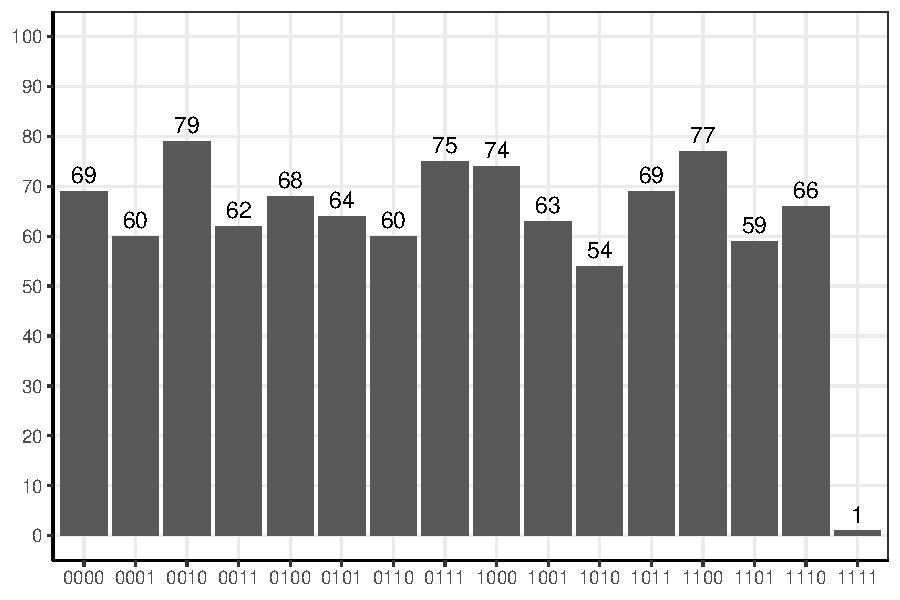
\includegraphics[width=\textwidth]{../../graphs/graph_numeric_histogram.pdf}
    \captionof{figure}{Histogram}
\end{minipage}

}


\frame{\frametitle{Generate synthetic data with CART (synthpop)}

\begin{minipage}{0.48\textwidth}
    \centering
    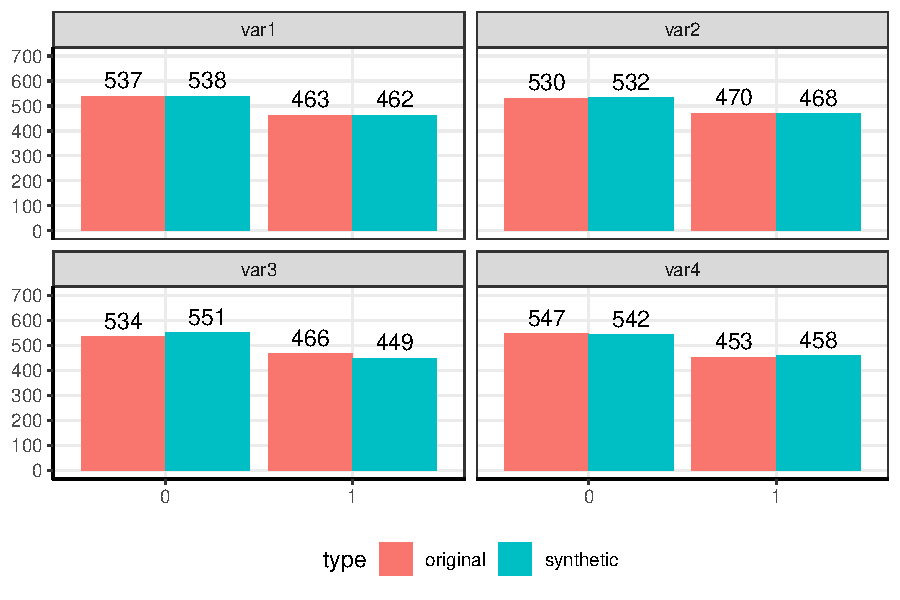
\includegraphics[width=\textwidth]{../../graphs/graph_numeric_compare_frequency.pdf}
    \captionof{figure}{Frequency}
\end{minipage}
\hfill
\begin{minipage}{0.48\textwidth}
    \centering
    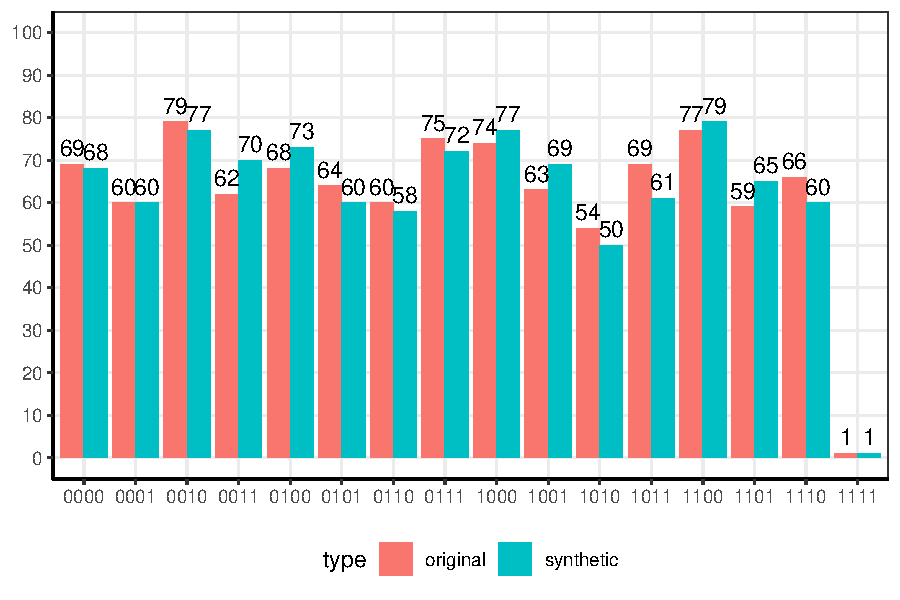
\includegraphics[width=\textwidth]{../../graphs/graph_numeric_compare_histogram.pdf}
    \captionof{figure}{Histogram}
\end{minipage}

}


\frame{\frametitle{Compare histogram x 100 synthetic datasets}
\begin{figure}
    \caption{Multiple synthetic data sets does not reduce privacy risk}
    \resizebox{\textwidth}{!}{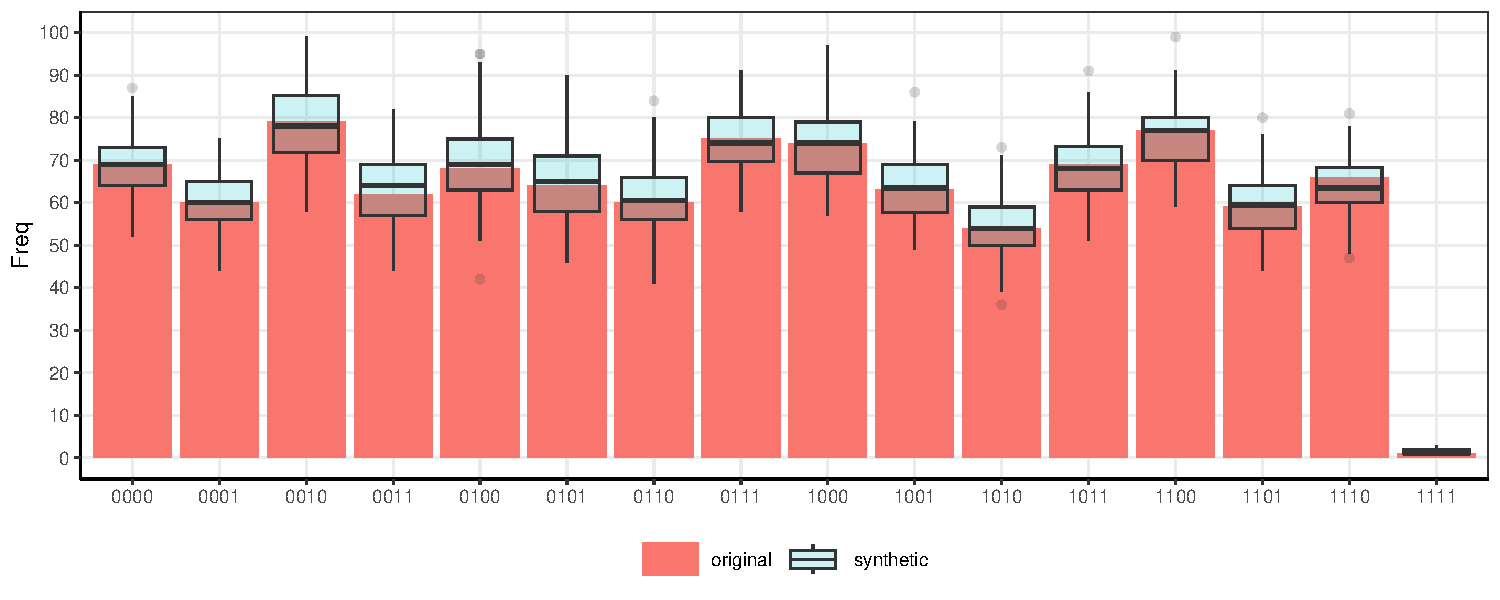
\includegraphics{../../graphs/graph_numeric_compare_histogram_100.pdf}}
    \label{fig:graph_numeric_compare_histogram_100}
\end{figure}
}

\frame{\frametitle{Describing the attack}
\begin{itemize}
    \item The attacker sees the synthetic data
    \item The attacker runs the same synthetic data model (SDG) for all of the 16 different possibilities.  
    \item Then they want to update their beliefs about what the last record could be
    \item The synthetic data contains that 16th category only in the case where the last observation is the unique one.
\end{itemize}
}


\frame{\frametitle{Illustrating the attack}
\vskip -3mm
\begin{figure}
    \caption{Histogram of 16 worlds x 100 synthetic datasets}
    \vskip -4mm
    \resizebox{\textwidth}{!}{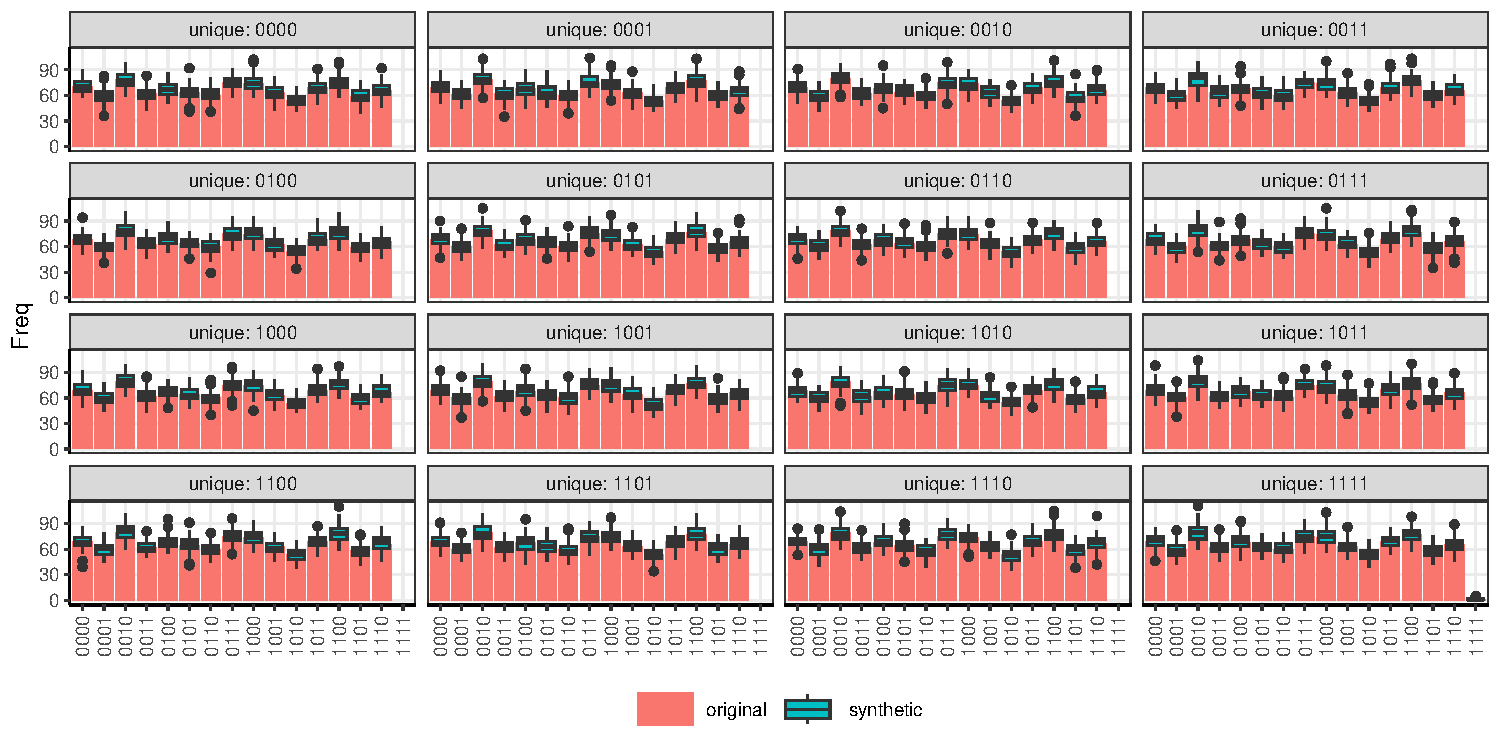
\includegraphics{../../graphs/graph_attacker.pdf}}
    \label{fig:graph_attacker}
\end{figure}
}


\frame{\frametitle{Summary}
\begin{itemize}
    \item The problem: CART can be disclosive 
    \item The reason: In our data, if a record is not in the original data, then it can never be in the synthetic data.  Therefore, a record can only be in the synthetic data if it is also in the original data.   
\end{itemize}
}


%%%%%%%%%%%%%%%%%%%%%%%%%%%%%%%%%%%%%%%%
%%%%%%%%%%%%%%%%%%%%%%%%%%%%%%%%%%%%%%%%
\section{Measuring privacy}\label{sec:privacy}
%%%%%%%%%%%%%%%%%%%%%%%%%%%%%%%%%%%%%%%%
%%%%%%%%%%%%%%%%%%%%%%%%%%%%%%%%%%%%%%%%
\begin{frame}[c,plain]
\vskip-4mm
\begin{beamercolorbox}[wd=\boxwidth,ht=22.11mm]{transparent}%
    \vfill%
    \usebeamerfont{title}%
    \leftinsert%
    \MakeUppercase{Section \ref{sec:privacy}: Measuring privacy
} % <- Hier die Überschrift eintragen
\end{beamercolorbox}
\vskip-3mm
\pgfuseimage{rahmenlinie}

What do the privacy metrics in Synthpop tells us?
\end{frame}


\frame{\frametitle{Privacy measures (synthpop - Raab et al., 2024)}
\begin{itemize}
    \item Identity disclosure: the ability to identify individuals in the data from a set of known characteristics (i.e. `keys').
    \item Attribute disclosure: the ability to find out from the keys something, not previously known
    \item Replicated uniques
\end{itemize}
}

\begin{frame}[fragile]
\frametitle{Comparing privacy measures (set.seed = 1237, i.e. unique = 1)}
  
% R Code block


\begin{minipage}[t]{0.48\textwidth}
\begin{lstlisting}
> print(t1, plot = FALSE, to.print = "ident")
Disclosure risk for 1000 records in the original data

Identity disclosure measures
from keys: var1 var2 var3 
For original  ( UiO )  0 %
For synthetic ( repU ) 0 %.
> print(t1, plot = FALSE, to.print = "attrib")

Table of attribute disclosure measures for var1 var2 var3 
Original measure is  Dorig and synthetic measure is DiSCO 
Variables Ordered by synthetic disclosure measure

       attrib.orig attrib.syn check1 Npairs check2
1 var4           0          0             0       
\end{lstlisting}
\end{minipage}%
  \hfill%
\begin{minipage}[t]{0.48\textwidth}
\begin{lstlisting}
> replicated.uniques (sds, df_ods)
    var1 var2 var3 var4
973    1    1    1    1
Uniques and replicated uniques for  1  synthesised data set(s)
 from keys:  var1 var2 var3 var4 

Uniques in  original data:
 1 from  1000 records ( 0.1 %) 
Uniques in synthetic data:
 1 from  1000 records ( 0.1% )

Replicated uniques:
 1
as a % of uniques in synthetic  100%
as a % of original records (repU) 0.1%
\end{lstlisting}
\end{minipage}
\end{frame}

\begin{frame}[fragile]
\frametitle{Comparing privacy measures (set.seed = 1240, i.e. unique = 3)}
  
% R Code block


\begin{minipage}[t]{0.48\textwidth}
\begin{lstlisting}
> print(t1, plot = FALSE, to.print = "ident")
Disclosure risk for 1000 records in the original data

Identity disclosure measures
from keys: var1 var2 var3 
For original  ( UiO )  0 %
For synthetic ( repU ) 0 %.
> print(t1, plot = FALSE, to.print = "attrib")

Table of attribute disclosure measures for var1 var2 var3 
Original measure is  Dorig and synthetic measure is DiSCO 
Variables Ordered by synthetic disclosure measure

       attrib.orig attrib.syn check1 Npairs check2
1 var4           0          0             0       
\end{lstlisting}
\end{minipage}%
  \hfill%
\begin{minipage}[t]{0.48\textwidth}
\begin{lstlisting}
> replicated.uniques (sds, df_ods)
Uniques and replicated uniques for  1  synthesised data set(s)
 from keys:  var1 var2 var3 var4 

Uniques in  original data:
 1 from  1000 records ( 0.1 %) 
Uniques in synthetic data:
 0 from  1000 records ( 0% )

Replicated uniques:
 0
as a % of uniques in synthetic  NaN%
as a % of original records (repU) 0%
\end{lstlisting}
\end{minipage}
\end{frame}

\frame{\frametitle{Summary}
\begin{itemize}
    \item Using common privacy measures, CART generates synthetic data with low risk
    \item 1 measure indicates there may be a problem, but all the other measures indicate there is no problem.
    \item However (and this is the point):
    \begin{itemize}
         \item We know there is a problem (because we created it)
         \item We know that common measures do not capture the problem 
     \end{itemize} 
     % \item We are also not alone in identifying this problem (Manrique-Vallier and Hu, 2018)
\end{itemize}
}


%%%%%%%%%%%%%%%%%%%%%%%%%%%%%%%%%%%%%%%%
%%%%%%%%%%%%%%%%%%%%%%%%%%%%%%%%%%%%%%%%
\section{Solution}\label{sec:solution}
%%%%%%%%%%%%%%%%%%%%%%%%%%%%%%%%%%%%%%%%
%%%%%%%%%%%%%%%%%%%%%%%%%%%%%%%%%%%%%%%%
\begin{frame}[c,plain]
\vskip-4mm
\begin{beamercolorbox}[wd=\boxwidth,ht=22.11mm]{transparent}%
    \vfill%
    \usebeamerfont{title}%
    \leftinsert%
    \MakeUppercase{Section \ref{sec:solution}: Solution
} % <- Hier die Überschrift eintragen
\end{beamercolorbox}
\vskip-3mm
\pgfuseimage{rahmenlinie}

\begin{itemize}
    \item The good news: we know how to solve the problem
    \item The bad news: we don't know how to identify the problem
\end{itemize}


\end{frame}

\frame{\frametitle{The good news: solutions}
\begin{itemize}
    \item cp = 0.05 (default = 1e$^{-8}$): prevent large trees (i.e. overfitting)
    \item minbucket = 75 (default = 5): the minimum number of observations in any terminal node
    \item Other options also exist
\end{itemize}
}

\frame{\frametitle{Compare histogram x 100 synthetic datasets}
\begin{minipage}{0.48\textwidth}
    \captionof{figure}{CART (default)}
    \resizebox{\textwidth}{!}{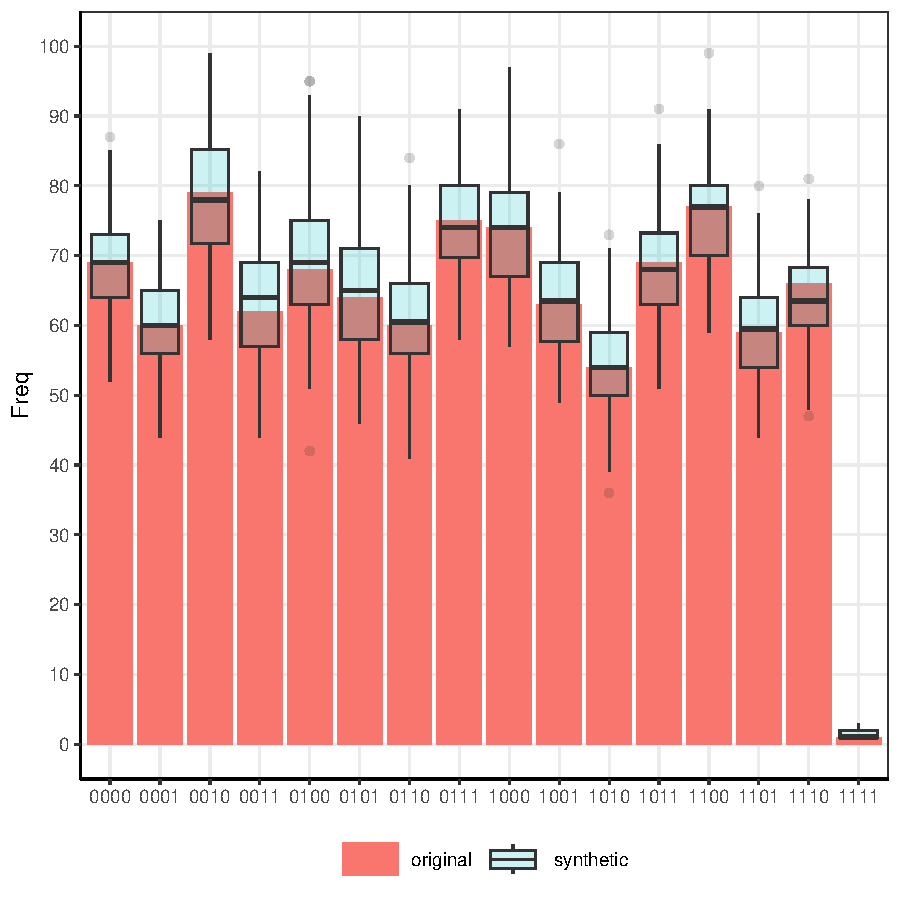
\includegraphics{../../graphs/graph_numeric_compare_histogram_100_v2.pdf}}
    \label{fig:graph_numeric_compare_histogram_100}
\end{minipage}
\hfill
\begin{minipage}{0.48\textwidth}
    \captionof{figure}{CART (modified)}
    \resizebox{\textwidth}{!}{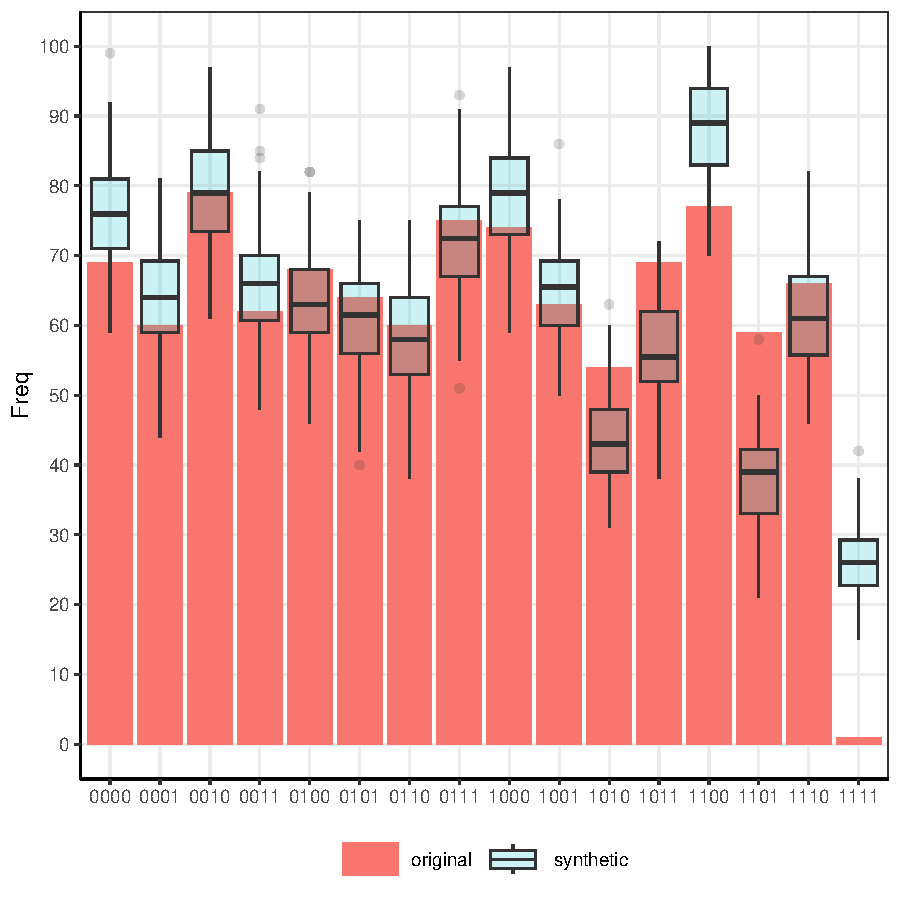
\includegraphics{../../graphs/graph_categorical_compare_histogram_100_v2.pdf}}
    \label{fig:graph_categorical_compare_histogram_100}
\end{minipage}
}

\frame{\frametitle{The bad news}
\begin{itemize}
    \item Specifically, we don't know how to identify the privacy risk
    \item Generally, we have to know a problem exists before we would do something about it
\end{itemize}
}

%%%%%%%%%%%%%%%%%%%%%%%%%%%%%%%%%%%%%%%%
%%%%%%%%%%%%%%%%%%%%%%%%%%%%%%%%%%%%%%%%
\section{Conclusion}\label{sec:conclusion}
%%%%%%%%%%%%%%%%%%%%%%%%%%%%%%%%%%%%%%%%
%%%%%%%%%%%%%%%%%%%%%%%%%%%%%%%%%%%%%%%%
\begin{frame}[c,plain]
\vskip-4mm
\begin{beamercolorbox}[wd=\boxwidth,ht=22.11mm]{transparent}%
    \vfill%
    \usebeamerfont{title}%
    \leftinsert%
    \MakeUppercase{Section \ref{sec:conclusion}: Conclusion} % <- Hier die Überschrift eintragen
\end{beamercolorbox}
\vskip-3mm
\pgfuseimage{rahmenlinie}
\end{frame}


\frame{\frametitle{Conclusion}
\begin{itemize}
    \item It has long been understood that there is a trade-off between utility and risk
    \item Previous research indicated that CART models were less sensitive to this trade-off than other SDGs 
    \item Using a simulated data set, we show that CART are sensitive to this trade-off
    \item The good news: It is possible to reduce risk in CART with parameters
    \item The bad news: 
    \begin{itemize}
        \item We must sacrifice utility
        \item Common privacy metrics do not capture risk in our simulated data
    \end{itemize}
    \item Question: If you did not know there was a problem, why would you sacrifice utility?

\end{itemize}
}

\frame{\frametitle{Contact}
Jonathan Latner \\
\url{jonathan.latner@iab.de} \\

Reproducible code: 
\begin{itemize}
    \item Github: \url{https://github.com/jonlatner/KEM\_GAN/tree/main/latner/projects/simulation} 
\end{itemize}
}



\end{spacing}
\end{document}

